\section{Generating Successors}
\label{sec::successors}
The successors of a search node $(I, r)$ are found by computing intervals from
the set of traversable points located on the same row of the grid as $I$ and
on the rows immediately adjacent.  
Whenever we generate a successor $(I', r')$ we want to guarantee that:
\begin{enumerate}
\item The local path from $r$ to $r'$ and then to each point $p' \in I'$ is taut.
\item The local path from $r$ to $r'$ and then to each point $p' \in I'$  does not pass
through any interval except $I$ and $I'$.
\end{enumerate}

We will distinguish between two kinds of successors: observable and non-observable. 

\subsection{Observable Successors}
A search node $(I', r')$ is an observable successor of $(I, r)$ if every 
$p' \in I'$ is visible from $r$ through $I$.
We compute observable successors as follows:

\begin{itemize}
\item If $I$ and $r$ are located on the same row of the grid, we construct a
a new \emph{closed interval} $I'$ that begins at the endpoint of $I$ farthest from $r$.
We extend $I'$ away from $r$ using the procedure described in in Section~\ref{sec::intervals}.
The new successor node is formed by the tuple $I'$ and the root point $r' = r$.
Figure~\ref{fig::anya_example} (Left) shows an example.
\item If $I$ and $r$ are located on different rows of the grid, we project $r$ through $I$
and construct a new \emph{closed interval} on the next row of the grid (moving away from $r$).
The new interval, which we call $I'$, contains only points that (i) are visible from $r$ through $I$
and that (ii) that can be reached from $r$ via a local path that is taut. 
The new successor node is formed by the tuple $I'$ and the root point $r' = r$.
\end{itemize}

There are many ways to implement the projection of the root point $r$ though the interval $I$
and onto the next row of the grid.
One simple method is to compute the endpoints of the new interval $I'$ by extending the
vectors $\vec{ra}$ and $\vec{rb}$ until they intersect the next row of the grid. 
Here $r$ is once more the root point and $a$ and $b$ are the endpoints of $I$.
The result of this operation is one or more observable successors, depending on whether or
not the interval $I'$ needs to split due to internal corner points.
Figure~\ref{fig::observable} (Middle) shows an example. 
In some cases the extension of one 
vector may be impeded by obstacles. When this occurs we can simply follow the contour of
the obstacle up to the next row of the grid. Figure~\ref{fig::observable} (Right) shows
an example.  


\begin{figure}[tb]
\center
		   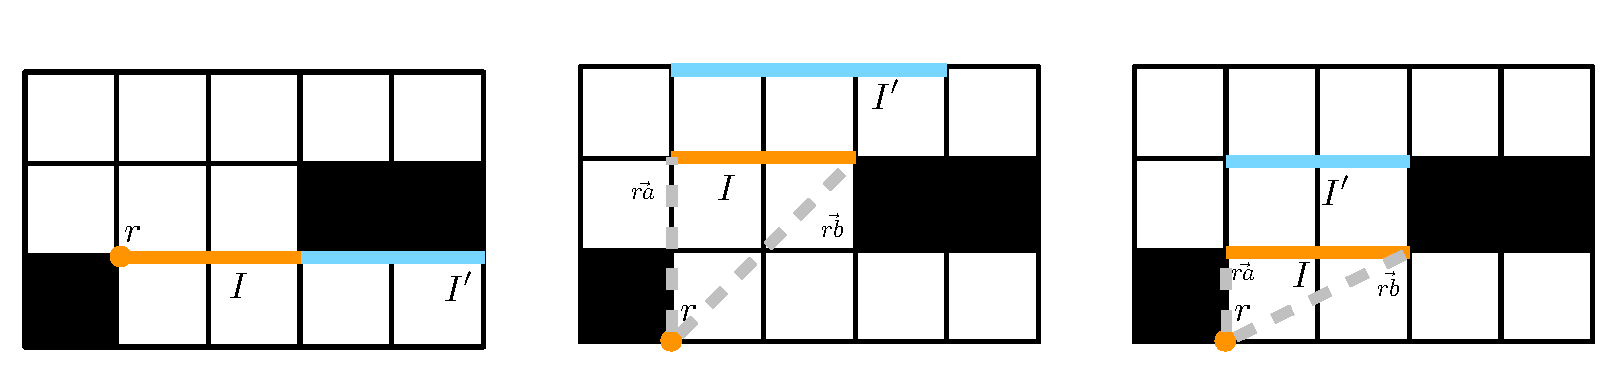
\includegraphics[width=\columnwidth]
			{images/observable.pdf}
	\vspace{-3pt}
\caption{\small
Examples of observable successors. In each case the current node is formed by the tuple $(I, r)$; the observable
successor is formed by the tuple $(I', r' = r)$. \textbf{(Left)} The root and interval of the current node $(I, r)$ are on
the same row. \textbf{(Middle)} Projecting $r$ through $I$ onto the next row of the grid. We extend the vectors $\vec{ra}$ and $\vec{rb}$
until they intersect the next row. The points of intersection become the endpoints of the closed interval $I'$. 
\textbf{(Right)} Alternative projection of $r$ through $I$ (due to obstacles).
}
\label{fig::observable}
\end{figure}

\subsection{Non-observable successors}
A search node $(I', r')$ is a non-observable successor of $(I, r)$ if $r'$ is visible from $r$ but
there exists no point $p' in I'$ which is visible from $r$ through $I$. There are two places
where we can find non-observable successors: (i) adjacent to the interval $I$; (ii) adjacent to the 
observable successors of $(I, r)$.

The following procedure describes in broad terms how to find non-observable successors 
among the points directly adjacent to the interval $I$.
\begin{enumerate}
\item Check if $I$ has at least one endpoint which is also a corner point. If
there exists no such endpoint, there are no non-observable successors and we
terminate. Otherwise:
\item Let $a$ be the endpoint of $I$ which is also a corner point (repeat the
following process if the other endpoint of $I$ is also a corner point).
\item If $r$ and $a$ are on the same row, follow the contour of the obstacle;
moving away from $a$ until we reach the next row. Starting from this point
(call it $a'$) we now construct a set of adjacent and closed intervals which
are all fully visible from $a$.  The combination of each of these intervals,
together with the common root point $r' = a$, form a set of non-observable
successors of $(I,r$). Figure~\ref{fig::non-observable} (Left) shows an
example.
\item If $r$ and $a$ are not on the same row, construct a new interval $I' =
(a, b]$ where $b$ is the next corner point or obstacle. Notice that $I'$ is
open at the endpoint $a$.  Look for other intervals among the points adjacent
to $I'$. Each one of these intervals (if any) must be constructed s.t. they
are closed at both ends.  The combination of each of these intervals,
together with the common root point $r' = a$, form a set of non-observable
successors of $(I,r$). Figure~\ref{fig::non-observable} (Middle) shows an
example.
\end{enumerate}

Thus far we have only discussed how to identify non-observable successors for
the node $(I, r)$ by searching among the points directly adjacent to the
interval $I$. We may also find non-observable successors by searching among
the points directly adjacent to some of the observable successors of $(I, r)$.
This procedure is identical Step 3 above. Simply substitute $I$ with the
approrpriate interval from an observable successor.
Figure~\ref{fig::non-observable} (Right) shows an example.

\begin{figure}[tb]
\center
		   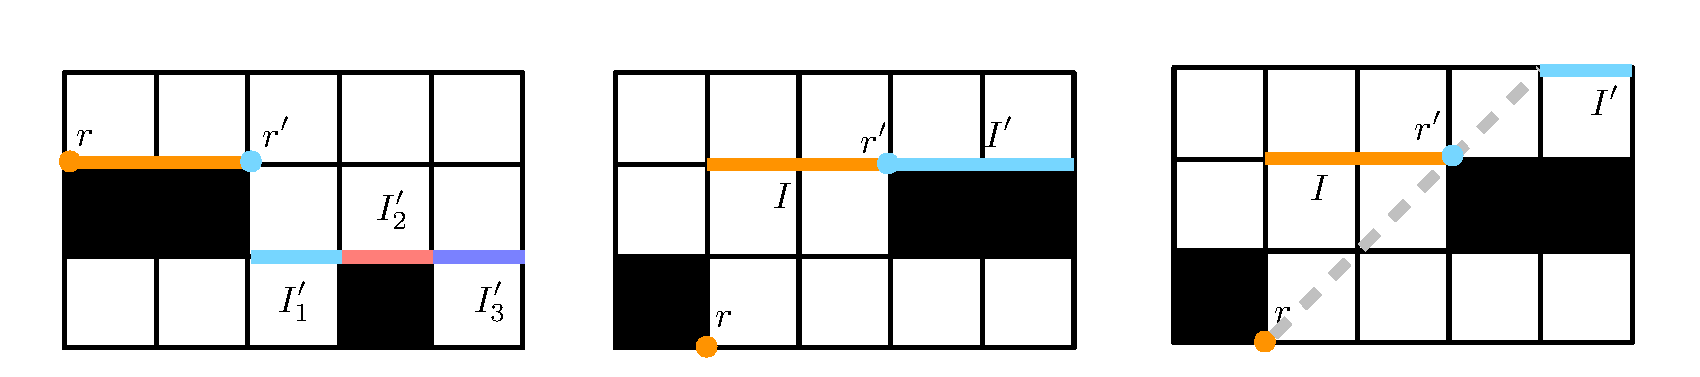
\includegraphics[width=\columnwidth]
			{images/non_observable.pdf}
	\vspace{-3pt}
\caption{\small
Examples of non-observable successors. In each case the current node
is formed by the tuple $(I, r)$; the non-observable successor 
is formed by the tuple $(I', r')$. If there is more than one 
non-observable successor we use a subscript index to distinguish them.
\textbf{(Left)} Non-observable successors when both $I$ and $r$ are on
the same row. \textbf{(Middle)} Non-observable successors among the 
points adjacent to $I$. \textbf{(Right)} Non-observable successors
adjacent to the points visible from $r$ through $I$.
}
\label{fig::non-observable}
\end{figure}
